\documentclass[a4paper]{article}

%=========================================
% Packages
%=========================================
\usepackage{mathtools}
\usepackage{amsfonts}
\usepackage{amsmath}
\usepackage{amssymb}
\usepackage{amsthm}
\usepackage[a4paper, total={6in, 8in}, margin=1in]{geometry}
\usepackage[utf8]{inputenc}
\usepackage{fancyhdr}
\usepackage[utf8]{inputenc}
\usepackage{graphicx}
\usepackage{physics}
\usepackage[listings]{tcolorbox}
\usepackage{hyperref}
\usepackage{tikz-cd}
\usepackage{adjustbox}
\usepackage{enumitem}
\usepackage[font=small,labelfont=bf]{caption}
\usepackage{subcaption}
\usepackage{wrapfig}
\usepackage{makecell}



\raggedright

\usetikzlibrary{arrows.meta}

\DeclarePairedDelimiter\ceil{\lceil}{\rceil}
\DeclarePairedDelimiter\floor{\lfloor}{\rfloor}

%=========================================
% Fonts
%=========================================
\usepackage{tgpagella}
\usepackage[T1]{fontenc}


%=========================================
% Custom Math Operators
%=========================================
\DeclareMathOperator{\adj}{adj}
\DeclareMathOperator{\im}{im}
\DeclareMathOperator{\nullity}{nullity}
\DeclareMathOperator{\sign}{sign}
\DeclareMathOperator{\dom}{dom}
\DeclareMathOperator{\lcm}{lcm}
\DeclareMathOperator{\ran}{ran}
\DeclareMathOperator{\ext}{Ext}
\DeclareMathOperator{\dist}{dist}
\DeclareMathOperator{\diam}{diam}
\DeclareMathOperator{\aut}{Aut}
\DeclareMathOperator{\inn}{Inn}
\DeclareMathOperator{\syl}{Syl}
\DeclareMathOperator{\edo}{End}
\DeclareMathOperator{\cov}{Cov}
\DeclareMathOperator{\vari}{Var}
\DeclareMathOperator{\cha}{char}
\DeclareMathOperator{\Span}{span}
\DeclareMathOperator{\ord}{ord}
\DeclareMathOperator{\res}{res}
\DeclareMathOperator{\Hom}{Hom}
\DeclareMathOperator{\Mor}{Mor}
\DeclareMathOperator{\coker}{coker}
\DeclareMathOperator{\Obj}{Obj}
\DeclareMathOperator{\id}{id}
\DeclareMathOperator{\GL}{GL}
\DeclareMathOperator*{\colim}{colim}

%=========================================
% Custom Commands (Shortcuts)
%=========================================
\newcommand{\CP}{\mathbb{CP}}
\newcommand{\GG}{\mathbb{G}}
\newcommand{\F}{\mathbb{F}}
\newcommand{\N}{\mathbb{N}}
\newcommand{\Q}{\mathbb{Q}}
\newcommand{\R}{\mathbb{R}}
\newcommand{\C}{\mathbb{C}}
\newcommand{\E}{\mathbb{E}}
\newcommand{\Prj}{\mathbb{P}}
\newcommand{\RP}{\mathbb{RP}}
\newcommand{\T}{\mathbb{T}}
\newcommand{\Z}{\mathbb{Z}}
\newcommand{\A}{\mathbb{A}}
\renewcommand{\H}{\mathbb{H}}
\newcommand{\K}{\mathbb{K}}

\newcommand{\mA}{\mathcal{A}}
\newcommand{\mB}{\mathcal{B}}
\newcommand{\mC}{\mathcal{C}}
\newcommand{\mD}{\mathcal{D}}
\newcommand{\mE}{\mathcal{E}}
\newcommand{\mF}{\mathcal{F}}
\newcommand{\mG}{\mathcal{G}}
\newcommand{\mH}{\mathcal{H}}
\newcommand{\mI}{\mathcal{I}}
\newcommand{\mJ}{\mathcal{J}}
\newcommand{\mK}{\mathcal{K}}
\newcommand{\mL}{\mathcal{L}}
\newcommand{\mM}{\mathcal{M}}
\newcommand{\mO}{\mathcal{O}}
\newcommand{\mP}{\mathcal{P}}
\newcommand{\mS}{\mathcal{S}}
\newcommand{\mT}{\mathcal{T}}
\newcommand{\mV}{\mathcal{V}}
\newcommand{\mW}{\mathcal{W}}

%=========================================
% Colours!!!
%=========================================
\definecolor{LightBlue}{HTML}{2D64A6}
\definecolor{ForestGreen}{HTML}{4BA150}
\definecolor{DarkBlue}{HTML}{000080}
\definecolor{LightPurple}{HTML}{cc99ff}
\definecolor{LightOrange}{HTML}{ffc34d}
\definecolor{Buff}{HTML}{DDAE7E}
\definecolor{Sunset}{HTML}{F2C57C}
\definecolor{Wenge}{HTML}{584B53}
\definecolor{Coolgray}{HTML}{9098CB}
\definecolor{Lavender}{HTML}{D6E3F8}
\definecolor{Glaucous}{HTML}{828BC4}
\definecolor{Mauve}{HTML}{C7A8F0}
\definecolor{Darkred}{HTML}{880808}
\definecolor{Beaver}{HTML}{9A8873}
\definecolor{UltraViolet}{HTML}{52489C}



%=========================================
% Theorem Environment
%=========================================
\tcbuselibrary{listings, theorems, breakable, skins}

\newtcbtheorem[number within = subsection]{thm}{Theorem}%
{	colback=Buff!3, 
	colframe=Buff, 
	fonttitle=\bfseries, 
	breakable, 
	enhanced jigsaw, 
	halign=left
}{thm}

\newtcbtheorem[number within=subsection, use counter from=thm]{defn}{Definition}%
{  colback=cyan!1,
    colframe=cyan!50!black,
	fonttitle=\bfseries, breakable, 
	enhanced jigsaw, 
	halign=left
}{defn}

\newtcbtheorem[number within=subsection, use counter from=thm]{axm}{Axiom}%
{	colback=red!5, 
	colframe=Darkred, 
	fonttitle=\bfseries, 
	breakable, 
	enhanced jigsaw, 
	halign=left
}{axm}

\newtcbtheorem[number within=subsection, use counter from=thm]{prp}{Proposition}%
{	colback=LightBlue!3, 
	colframe=Glaucous, 
	fonttitle=\bfseries, 
	breakable, 
	enhanced jigsaw, 
	halign=left
}{prp}

\newtcbtheorem[number within=subsection, use counter from=thm]{lmm}{Lemma}%
{	colback=LightBlue!3, 
	colframe=LightBlue!60, 
	fonttitle=\bfseries, 
	breakable, 
	enhanced jigsaw, 
	halign=left
}{lmm}

\newtcbtheorem[number within=subsection, use counter from=thm]{crl}{Corollary}%
{	colback=LightBlue!3, 
	colframe=LightBlue!60, 
	fonttitle=\bfseries, 
	breakable, 
	enhanced jigsaw, 
	halign=left
}{crl}

\newtcbtheorem[number within=subsection, use counter from=thm]{eg}{Example}%
{	colback=Beaver!5, 
	colframe=Beaver, 
	fonttitle=\bfseries, 
	breakable, 
	enhanced jigsaw, 
	halign=left
}{eg}

\newtcbtheorem[number within=subsection, use counter from=thm]{ex}{Exercise}%
{	colback=Beaver!5, 
	colframe=Beaver, 
	fonttitle=\bfseries, 
	breakable, 
	enhanced jigsaw, 
	halign=left
}{ex}

\newtcbtheorem[number within=subsection, use counter from=thm]{alg}{Algorithm}%
{	colback=UltraViolet!5, 
	colframe=UltraViolet, 
	fonttitle=\bfseries, 
	breakable, 
	enhanced jigsaw, 
	halign=left
}{alg}




%=========================================
% Hyperlinks
%=========================================
\hypersetup{
    colorlinks=true, %set true if you want colored links
    linktoc=all,     %set to all if you want both sections and subsections linked
    linkcolor=DarkBlue,  %choose some color if you want links to stand out
}


\pagestyle{fancy}
\fancyhf{}
\rhead{Labix}
\lhead{Topological Manifolds}
\rfoot{\thepage}

\title{Topological Manifolds}

\author{Labix}

\date{\today}
\begin{document}
\maketitle
\begin{abstract}
\end{abstract}
\pagebreak
\tableofcontents
\pagebreak

\section{Structural Theorems of Topological Manifolds}
\subsection{Triangulable Manifolds}
\begin{defn}{Triangulable Manifolds}{} Let $M$ be a $k$-manifold. We say that $M$ is triangulable if $M$ is a $\delta$-complex structure consisting of a finite number of top simplicies. 
\end{defn}

\begin{prp}{}{} Every finite CW complex is homotopy equivalent to a topological manifold. 
\end{prp}

\subsection{Topological, Piecewise Linear and Smooth Manifolds}

\subsection{Covering Spaces of Manifolds}
\begin{prp}{}{} Let $M$ be a manifold. Let $p:\widetilde{M}\to M$ be a covering space. Then $\widetilde{M}$ is also a manifold. 
\end{prp}

\subsection{General Homological Results of Manifolds}
\begin{lmm}{}{} Let $M$ be a connected $k$-dimensional manifold. Let $R$ be a ring. Then we have $$H_i(M;R)=0$$ for all $i\geq k$. 
\end{lmm}

The remainder of the subsection concerns compact manifolds. 

\begin{prp}{}{} Let $M$ be a compact manifold. Then $H_k(M)$ is finitely generated for all $k\in\N$. 
\end{prp}

\begin{prp}{}{} Let $M$ be a compact manifold. If $\dim(M)$ is odd, then $\chi(M)=0$. 
\end{prp}

\pagebreak
\section{Orientability of a Topological Manifold}
\subsection{Local and Global Orientations}
The key observation in defining orientation through homology is the following proposition, which shows that the local homology groups on a manifold are isomorphic to $R$ on the top dimension. 

\begin{prp}{}{} Let $M$ be a $k$-dimensional topological manifold and $x\in M$ a point. Let $R$ be a ring. Then $$H_n(M\;|\;\{x\};R)\cong\begin{cases}
R & \text{ if } n=k\\
0 & \text{ otherwise }
\end{cases}$$ \tcbline
\begin{proof}
Let $x\in M$. Since $M$ is a manifold, there exists an open neighbourhood of $x$ such that $U\cong\R^k$ via some transition map $\varphi:U\to\R^k$. Since $M\setminus U$ is closed, we can apply excision to obtain an isomorphism $$H_n(M\;|\;\{x\};R)\cong H_n(U\;|\;\{x\};R)$$ By the homeomorphism $(U,U\setminus\{x\})\cong(\R^k,\R^k\setminus\{\varphi(x)\})$ and 6.3.2 in AT2, we obtain the desired result. 
\end{proof}
\end{prp}

\begin{defn}{Local Orientation}{} Let $M$ be a $k$-dimensional topological manifold and let $x\in M$. A local orientation of $M$ at $x$ is a choice of generator of $$H_k(M\;|\;\{x\};R)\cong R$$
\end{defn}

Notice that being a generator of $R$ is the same as saying that it is a unit of $R$. 

\begin{defn}{Open and Closed Ball in Manifolds}{} Let $M$ be a $k$-dimensional topological manifold and let $(U,\varphi)$ be a chart of $M$. We say that $B\subset U$ is an open / closed ball if $\varphi(B)\subseteq\R^k$ is an open / closed ball of $\R^k$. 
\end{defn}

The point of the definition is that we have the following. We have homotopy equivalences \\~\\
\adjustbox{scale=1.0,center}{\begin{tikzcd}
	& {(\R^k,\R^k\setminus B)} \\
	{(\R^k,\R^k\setminus\{x\})} && {(\R^k,\R^k\setminus\{y\})}
	\arrow["\simeq", from=2-1, to=1-2]
	\arrow["\simeq"', from=2-3, to=1-2]
\end{tikzcd}}\\~\\
given by deformation retracts. If $M$ is a $k$-manifold and $U\subseteq M$ is an open ball, we can use excision to obtain isomorphisms \\~\\
\adjustbox{scale=1.0,center}{\begin{tikzcd}
	& {H_k(M\;|\;U)} \\
	{H_k(M\;|\;\{x\})} && {H_k(M\;|\;\{y\})}
	\arrow["\cong"', from=1-2, to=2-1]
	\arrow["\cong", from=1-2, to=2-3]
\end{tikzcd}}\\~\\
All of the above groups are just $\Z$, and a choice of local orientation is a choice of generators of the lower two homology groups. If we want the choice to be consistent, then we better have the two generators coincide to the same generator in $H_n(M\;|\;U)$ under the above isomorphisms. We note here that the isomorphism $$H_n(M\;|\;U)\overset{\cong}{\longrightarrow}H_n(M\;|\;\{x\})$$ for any $x\in U$ came from the inclusion map $(M,M\setminus U)\hookrightarrow(M,M\setminus\{x\})$. 

If $M$ is a $k$-manifold and $U\subseteq M$ is an open ball, a similar argument as the case of $R=\Z$ shows that there are isomorphisms \\~\\
\adjustbox{scale=1.0,center}{\begin{tikzcd}
	& {H_k(M\;|\;U;R)} \\
	{H_k(M\;|\;\{x\};R)} && {H_k(M\;|\;\{y\};R)}
	\arrow["\cong"', from=1-2, to=2-1]
	\arrow["\cong", from=1-2, to=2-3]
\end{tikzcd}}\\~\\
where all of the above groups are just $R$. We also obtain the same definition for consistent local orientations. 

\begin{defn}{Consistent Local Orientations}{} Let $M$ be a $k$-manifold. Let $B$ be an open ball in $M$. For each $x\in B$, let $\omega_x$ be a choice of local orientation at $x$. We say that the choices of local orientations at $B$ is consistent if there exists a generator $\omega_B\in H_k(M\;|\; B;R)$ such that for any $x,y\in B$, under the isomorphisms \\~\\
\adjustbox{scale=1.0,center}{\begin{tikzcd}
	{H_k(M\;|\;\{x\};R)} & {H_k(M\;|\;B;R)} & {H_k(M\;|\;\{y\};R)} \\
	{\omega_x} & {\omega_B} & {\omega_y}
	\arrow["\cong", from=1-1, to=1-2]
	\arrow["\cong"', from=1-3, to=1-2]
	\arrow[maps to, from=2-1, to=2-2]
	\arrow[maps to, from=2-3, to=2-2]
\end{tikzcd}}\\~\\
the choice of local orientation maps to the same generator $\omega_B$. 
\end{defn}

\begin{defn}{R-Orientation of a Manifold}{} Let $M$ be a $k$-dimensional topological manifold. An orientation of $M$ is a function $$x\mapsto\omega_x\in H_k(M,M\setminus\{x\};R)$$ assigning every point to a local orientation such that for every $x\in M$, there exists an open ball $x\in B$ such that $(\omega_x)_{x\in B}$ a consistent local orientation. 
\end{defn}

\subsection{The Orientation Bundle}
\begin{defn}{Orientation Bundle}{} Let $M$ be a topological manifold. Define the orientation bundle $\widetilde{M}$ to be the set of pairs $$\widetilde{M}=\left\{(x,\omega_x)\;\bigg{|}\;\; x\in M, \omega_x\text{ is a generator of }H_k(M\;|\; x)\right\}$$ together the projection map $\pi:\widetilde{M}\to M$ defined by $\pi(x,\omega_x)=x$. 
\end{defn}

\begin{defn}{Topology on the Orientation Bundle}{} Let $M$ be a topological manifold. Define the topology on the orientation bundle $\widetilde{M}$ as follows. Let $B$ be an open ball in $M$. Since there are exactly two distinct orientation classes on $B$ we have that $$\pi^{-1}(B)=B_+\amalg B_-$$ where $B_+$ and $B_-$ are homeomorphic to $B$. Define the topology of $\widetilde{M}$ to be generated by sets of the form $B_+$ and $B_-$. 
\end{defn}

\begin{lmm}{}{} For any topological manifold $M$, $\widetilde{M}$ is a manifold and is a $2$-sheeted covering. \tcbline
\begin{proof}
Let $(x,\omega_x)$ and $(y,\omega_y)$ in $\widetilde{M}$ be distinct. If $x=y$ then $\omega_x=-\omega_y$. We know that there are two distinct orientation classes so $\pi^{-1}$ is a disjoint union consisting of those with positive orientation and those with negative. Since $\omega_x$ and $\omega_y$ are opposite, they lie in the disjoint union separately so that they are disjoint. If $x\neq y$, then since $M$ is Hausdorff then we can choose $U_1$ and $U_2$ disjoint neighbourhoods of $x$ and $y$ respectively. Then this means that $\pi^{-1}(U_1)$ and $\pi^{-1}(U_2)$ are disjoint. Thus we have shown that $M$ is Hausdorff. \\~\\

Now let $(x,\omega_x)\in\widetilde{M}$. Then since $M$ is manifold, there is an open ball $B$ around $x$ so that $B$ is homeomorphic to $\R^k$. $\pi^{-1}(B)$ is then a disjoint union of two copies of $B$, one such copy contains $(x,\omega_x)$. Then we have found a neighbourhood for $(x,\omega_x)$ that is homeomorphic to $\R^k$. Thus we are done. \\~\\

It is clear that it is a two sheeted covering because for any open set $B\subseteq M$, $\pi^{-1}(B)=B_+\amalg B_-$. 
\end{proof}
\end{lmm}

\begin{lmm}{}{} Let $M$ be a topological $k$-manifold. Then the orientation bundle $\widetilde{M}$ is orientable. \tcbline
\begin{proof}
Suppose that $(x,\omega_x)$ and $(y,\omega_y)$ in $\widetilde{M}$ share an open ball $\widetilde{B}$ of $\widetilde{M}$. By definition of $\widetilde{M}$, the topology is generated by $\pi^{-1}(B)=B_+\amalg B_-$ for any open ball $B$ of $M$. Hence any open ball of $\widetilde{M}$ must be equal to some $B_+$ or $B_-$. Without loss of generality, suppose that $B$ is an open ball of $M$ such that $\widetilde{B}$ is one of $B_+$ or $B_-$ in $\pi^{-1}(B)$. Then $x$ and $y$ share an open ball $B$. We have seen the following isomorphisms induced by inclusions: \\~\\
\adjustbox{scale=1.0,center}{\begin{tikzcd}
	& {H_k(M\;|\;B)} \\
	{H_k(M\;|\;x)} & {H_k(\widetilde{M}\;|\;\widetilde{B})} & {H_k(M\;|\;y)} \\
	{H_k(\widetilde{M}\;|\;(x,\omega_x))} && {H_k(\widetilde{M}\;|\;(y,\omega_y))}
	\arrow["\cong", from=2-1, to=1-2]
	\arrow["\cong"', from=2-3, to=1-2]
	\arrow["\cong", from=3-1, to=2-2]
	\arrow["\cong"', from=3-3, to=2-2]
\end{tikzcd}}\\~\\
By excision, we can connect the above diagram with isomorphisms: \\~\\
\adjustbox{scale=1.0,center}{\begin{tikzcd}
	& {H_k(M\;|\;B)} \\
	{H_k(M\;|\;x)} & {H_k(\widetilde{M}\;|\;\widetilde{B})} & {H_k(M\;|\;y)} \\
	{H_k(\widetilde{M}\;|\;(x,\omega_x))} && {H_k(\widetilde{M}\;|\;(y,\omega_y))}
	\arrow["\cong", from=2-1, to=1-2]
	\arrow["\cong"{description}, from=2-2, to=1-2]
	\arrow["\cong"', from=2-3, to=1-2]
	\arrow["\cong"{description}, from=3-1, to=2-1]
	\arrow["\cong", from=3-1, to=2-2]
	\arrow["\cong"', from=3-3, to=2-2]
	\arrow["\cong"{description}, from=3-3, to=2-3]
\end{tikzcd}}\\~\\
By definition of $\pi^{-1}(B)=B_+\amalg B_-$, if $(x,\omega_x)$ and $(y,\omega_y)$ lie in the same ball, they have a consistent local orientation. Hence there exists a generator $\omega_B$ of $H_k(M\;|\;B)$ such that the above diagram maps elements in the following way: \\~\\
\adjustbox{scale=1.0,center}{\begin{tikzcd}
	& {\omega_B} \\
	{\omega_x} && {\omega_y}
	\arrow[maps to, from=2-1, to=1-2]
	\arrow[from=2-3, to=1-2]
\end{tikzcd}}\\~\\
Under the isomorphism $H_k(M\;|\;x)\cong H_k(\widetilde{M}\;|\;(x,\omega_x))$ let $\omega_x$ be sent to the generator $\mu_{(x,\omega_x)}$. Define $\mu_{(y,\omega_y)}$ and $\mu_{\widetilde{B}}$ similarly. Then using the above diagram with 6 local homology groups, we can see that elements are sent in the following way: \\~\\
\adjustbox{scale=1.0,center}{\begin{tikzcd}
	& {\omega_B} \\
	{\omega_x} & {\mu_{\widetilde{B}}} & {\omega_y} \\
	{\mu_{(x,\omega_x)}} && {\mu_{(y,\omega_y)}}
	\arrow[maps to, from=1-2, to=2-2]
	\arrow[maps to, from=2-1, to=1-2]
	\arrow[from=2-3, to=1-2]
	\arrow[maps to, from=3-1, to=2-1]
	\arrow[dashed, maps to, from=3-1, to=2-2]
	\arrow[dashed, maps to, from=3-3, to=2-2]
	\arrow[maps to, from=3-3, to=2-3]
\end{tikzcd}}\\~\\
This show that we made a choice of generators for the local homology groups of $\widetilde{M}$ for which they are consistent (they both map to the same generator $\mu_{\widetilde{B}}$). Hence $\widetilde{M}$ is orientable. 
\end{proof}
\end{lmm}

In order to deduce interesting results, we need to define a more general version than that of the orientation double cover. 

\begin{defn}{Generalized Orientation Bundle}{} Let $M$ be a $k$-manifold. Let $R$ be a ring. Define the generalized orientation bundle $M_R$ of $M$ to be the set $$M_R=\{(x,\mu_r)\;|\;x\in M, r\in H_k(M\;|\; x;R)\cong R\}$$ together with the topology generated by each $B_r$ in $$\pi^{-1}(B)=\coprod_{r\in R\text{ is a unit}}B_r$$
\end{defn}

When $R=\Z$, we notice that $M_\Z\to M$ is infinite sheeted, and contains a copy of $M$ as the subspace of $M_\Z$ by choosing $\mu_r=0\in\Z$. More generally, if we write $$M_k=\{(x,\mu_x)\in M_\Z\;|\;\mu_x=\pm k\}$$ $M_\Z$ contains a copy of $M_k$ for $k\in\N\setminus\{0\}$, and each copy $M_k$ is homeomorphic to the orientation double cover $\widetilde{M}$. \\

If we instead consider an arbitrary ring $R$, then we can similarly define $$M_r=\left\{(x,\mu_x)\in M_R\;|\;\substack{\mu_x\otimes r\in H_k(M\;|\; x)\otimes R\cong H_k(M\;|\; x;R)\\\mu_x\text{ is a generator }H_k(M\;|\;x)\cong\Z}\right\}$$ If $2r=0$ in the ring then $M_r$ becomes only one copy of $M$. Otherwise for each $r\in R$, $M_r$ is homemorphic to $\widetilde{M}$. Hence the covering space $M_R$ is a disjoint union of $M_r$ for $r\in R$, except that $M_r$ and $M_{-r}$ are not disjoint. 

\begin{lmm}{}{} Let $M$ be a topological manifold. Let $R$ be a ring. Then $M$ is $R$-orientable if and only if there exists a section $M\to M_R$. In particular, the section is precisely the assignment required in the definition of $R$-orientability. \tcbline
\begin{proof}
Let $M$ be $R$-orientable. Then there exists an assignment $x\mapsto\omega_x\in H_k(M\;|\;x;R)$ for each $x\in M$. We can rewrite the assignment into $x\mapsto(x,\omega_x)$ so that the codomain is now $M_R$. It is clear that composing with the projection map gives the identity. It remains to show that the assignment is continuous. Since the topology of $M_R$ is generated by open balls, it suffices to check continuity on open balls. So let $\widetilde{B}$ be an open ball of $M_R$. It is clear that the preimage of $\widetilde{B}$ is given by $x\in M$ such that $(x,\omega_x)\in\widetilde{B}$. But this is the same set as $B=\pi(\widetilde{B})$, which by definition is an open ball. Hence $s$ is continuous. \\~\\

Now let $s:M\to M_R$ be a section. By restricting to the second factor we obtain an assignment $x\mapsto\omega_x\in H_k(M\;|\;x;R)$. I claim that defines an orientation. By continuity of $s$, the preimage of each open ball $\widetilde{B}$ of $M_R$ by $s$ is also an open ball $B$ of $M$. For $x,y\in B$, $\omega_x$ and $\omega_y$ is in $\widetilde{B}$. But $\widetilde{B}$ is one of the factors of the disjoint union $\pi^{-1}(B)=\coprod_{r\in R\text{ is a unit}}B_r$, which by definition consists of consistent local orientations. Hence $\omega_x$ and $\omega_y$ are consistent. Thus we conclude. 
\end{proof}
\end{lmm}

\begin{prp}{}{} Let $M$ be a connected topological manifold. Then the following are true. 
\begin{itemize}
\item $M$ is orientable if and only if $\widetilde{M}\cong M\amalg M$. In this case, $M$ admits exactly two possible orientations. 
\item $M$ is non-orientable if and only if $\widetilde{M}\to M$ is a non-trivial two sheeted cover. 
\end{itemize} \tcbline
\begin{proof}
Let $M$ first be orientable. Then there exists a section $s:M\to\widetilde{M}$ to the covering space. Assume for a contradiction that $\widetilde{M}$ is connected. Let $\gamma$ be a path from $(x,\omega_x)$ to $(x,-\omega_x)$. Then notice that $\gamma$ and $s\circ\pi\circ\gamma$ are distinct lifts of the path $\pi\circ\gamma$ in $M$. This contradicts the uniqueness of path lifting. Thus $\widetilde{M}$ is disconnected. The unique disconnected two sheeted cover of a space is precisely the disjoin union of the space. So we are done. \\~\\

Now let $\widetilde{M}\cong M\amalg M$. Then it is easy to see that there exists a section $s:M\to\widetilde{M}$ simply be mapping homeomorphically to one of the disjoint components. \\~\\

When $M$ is orientable, we have that $\widetilde{M}\cong M\amalg M$. By the above lemma, each section $M\to\widetilde{M}$ corresponds to one choice of orientation. There can only be two choices of distinct sections $M\to M\amalg M$. Hence $M$ has exactly two orientations. \\~\\

The second statement is precisely the contrapositive of the equivalent characterization of orientability. 
\end{proof}
\end{prp}

\begin{lmm}{}{} Let $M$ be a topological manifold. Let $R$ be a ring. Then the following are true. 
\begin{itemize}
\item If $M$ is orientable, then $M$ is $R$-orientable. 
\item If $M$ is non-orientable, then $M$ is $R$-orientable if and only if $R$ contains a unit of order $2$. 
\end{itemize}
\end{lmm}

\begin{defn}{Set of Sections}{} Let $M$ be a compact $k$-manifold. Denote $p:M_R\to M$ the projection map. Define the set of sections of $M$ to the orientation cover to be the set $$\Gamma(M,M_R)=\{s:M\to M_R\;|\;s\circ p=\text{id}_M\}$$
\end{defn}

\begin{prp}{}{} Let $M$ be a $k$-manifold. Let $K\subseteq M$ be compact. Then the following are true. 
\begin{itemize}
\item If $s:M\to M_R$ is a section sending $x$ to $(x,\mu_x)$, there exists a unique $\mu_K\in H_k(M\;|\;K;R)$ such that under induced map of inclusions $$H_k(M\;|\;K;R)\to H_k(M\;|\;x;R)$$ $\mu_K$ is mapped to $\mu_x$. 
\item The local homology groups $H_i(M\;|\;K;R)=0$ for all $i>k$. 
\end{itemize} \tcbline
\begin{proof}
Step 1: If the statement is true for compact subsets $A,B,A\cap B$, then it is true for $A\cup B$. \\
We obtain an exact sequence: \\~\\
\adjustbox{scale=1.0,center}{\begin{tikzcd}
	0 & {H_k(M\;|\;A\cup B;R)} & {H_k(M\;|\;A;R)\oplus H_k(M\;|\;B;R)} & {H_k(M\;|\;A\cap B;R)}
	\arrow[from=1-1, to=1-2]
	\arrow["\Phi", from=1-2, to=1-3]
	\arrow["\Psi", from=1-3, to=1-4]
\end{tikzcd}}\\~\\
using the Mayer Vietoris sequence. Since $H_i(M\;|\;A;R)$ and $H_i(M\;|\;B;R)$ is $0$ for all $i>k$, we conclude that $H_i(M\;|\;A\cup B;R)=0$ for all $i>k$. This proves the second half of the proposition. For the first half, let $s:M\to M_R$ be a section sending $x$ to $(x,\mu_x)$. Then we obtain unique classes $\mu_A\in H_k(M\;|\;A;R)$ and $\mu_B(M\;|\;;B;R)$ and $\mu_{A\cap B}\in H_k(M\;|\;A\cap B;R)$ such that for $x\in A\cap B$, $\mu_A$, $\mu_B$ and $\mu_{A\cap B}$ are all mapped to $\mu_x$ in the maps $$H_k(M\;|\;A;R),H_k(M\;|\;B;R),H_k(M\;|\;A\cap B;R)\to H_k(M\;|\;x;R)$$ Then $\Psi(\mu_A,-\mu_B)=\mu_{A\cap B}-\mu_{A\cap B}=0$ implies that $(\mu_A,-\mu_B)\in\ker(\Psi)$. By exactness of the above sequence, there exists $\mu_{A\cup B}\in H_k$ such that $\Phi(\mu_{A\cup B})=(\mu_A,-\mu_B)$. \\~\\

For uniqueness, suppose that $\mu_{A\cup B}$ and $\mu_{A\cup B}'$ be two such elements satisfying the requirements. Consider the following diagram: \\~\\
\adjustbox{scale=1.0,center}{\begin{tikzcd}
	0 & {H_k(M\;|\;A\cup B;R)} & {H_k(M\;|\;A;R)\oplus H_k(M\;|\;B;R)} & {H_k(M\;|\;A\cap B;R)} \\
	\\
	&& {H_k(M\;|\;x;R)}
	\arrow[from=1-1, to=1-2]
	\arrow["\Phi", from=1-2, to=1-3]
	\arrow[from=1-2, to=3-3]
	\arrow["\Psi", from=1-3, to=1-4]
	\arrow[from=1-3, to=3-3]
	\arrow[from=1-4, to=3-3]
\end{tikzcd}}\\~\\
It is commutative since $\Phi$ and $\Psi$ are induced by inclusions. Then the image of $\mu_{A\cap B}-\mu_{A\cap B}'$ is $0$ in $H_k(M\;|\;x;R)$. By commutativity of the left triangle, the image of $\mu_A-\mu_A'$ and $\mu_B-\mu_B'$ is $0$ in $H_k(M\;|\;x;R)$. Since $\Phi$ is injective, this implies that $\mu_{A\cap B}=\mu_{A\cap B}'$. \\~\\

Step 2: Reduce to the case of $M=\R^n$. \\
If $K\subseteq M$ is compact, then there exists compact subsets $K_1,\dots,K_n$ of $M$, each contained in a local chart and hence homeomorphic to a subset of $\R^n$, such that $K=K_1\cup\cdots\cup K_n$. By step 1, it sufficies to consider $K_1$. Then by excision, it sufficies to consider a compact subset $K$ of $\R^n$. \\~\\

Step 3: Reduce to the case of a convex compact subset of $\R^n$. \\
\end{proof}
\end{prp}

\begin{prp}{}{} Let $M$ be a compact $k$-manifold. Then the following are true. 
\begin{itemize}
\item If $M$ is $R$-orientable, then there is an $R$-module isomorphism $$\Gamma(M,M_R)\cong\Hom(\pi_0(M),R)$$ of sets. This assignment is given by sending $s:\pi_0(M)\to R$ to the map $x\mapsto(x,s([x]))$. 
\item If $M$ is connected and not $R$-orientable, then there are no global sections. 
\end{itemize}
\end{prp}

\begin{thm}{}{} Let $M$ be a compact and connected $k$-dimensional manifold. Let $R$ be a ring. Then the following are true. 
\begin{itemize}
\item If $M$ is $R$-orientable, then the map $$H_k(M;R)\to H_k(M\;|\;x;R)\cong R$$ is an isomorphism for all $x\in M$. 
\item If $M$ is not $R$-orientable, then the map $$H_k(M;R)\to H_k(M\;|\;x;R)\cong R$$ is injective and has image $\{r\in R\;|\;2r=0\}$ for all $x\in M$
\end{itemize}
\end{thm}

Notice this theorem is not a definitive criterion for orientability in general. However, if $R=\Z$, then it becomes a sufficient criterion. \\

We can summarize the situation as follows: $$M\text{ is orientable }\implies\substack{TFAE:\\M\text{ is }R\text{-orientable}\\\text{there exists a section }M\to M_R\\}\implies\substack{\Gamma(M,M_R)\cong\Hom(\pi_0(M),R)\\H_k(M;R)\cong H_k(M\;|\;x)\cong R}$$~

$$\substack{TFAE:\\M\text{ is not }R\text{-orientable}\\\text{there are no sections }M\to M_R\\}\implies\substack{H_k(M;R)\longrightarrow H_k(M\;|\;x)\cong R\text{ is injective}}$$

\subsection{Consequences of Orientability on Homology}
\begin{crl}{}{} Let $M$ be a compact and connected $k$-dimensional manifold. Then the following are true. 
\begin{itemize}
\item If $M$ is orientable, then the torsion part of $H_{k-1}(M)$ is trivial. 
\item If $M$ is not-orientable, then the torsion part of $H_{k-1}(M)$ is $\Z/2\Z$. 
\end{itemize}
\end{crl}

\begin{crl}{}{} Any simply connected manifold is orientable. \tcbline
\begin{proof}
By Galois theory of covering spaces, any $2$-sheeted cover of a simply connected space is disconnected. 
\end{proof}
\end{crl}

\begin{prp}{}{} Let $M,N$ be compact connected manifolds of dimension $n$. Then the following are true. 
\begin{itemize}
\item For $1\leq i\leq n-2$, we have $$H_i(M\# N)\cong H_i(M)\oplus H_i(N)$$
\item If one of $M$ or $N$ are orientable, then $$H_{n-1}(M\# N)\cong H_{n-1}(M)\oplus H_{n-1}(N)$$
\item If $M$ and $N$ are non-orientable, then $H_{n-1}(M\# N)$ is obtained from $H_{n-1}(M)\oplus H_{n-1}(N)$ by replacing one of the $\Z/2\Z$ summands with $\Z$. 
\end{itemize}
\end{prp}

\begin{lmm}{}{} Let $M,N$ be compact connected manifolds of dimension $n$. Then we have $$\chi(M_1\# M_2)=\chi(M_1)+\chi(M_2)-\chi(S^n)$$
\end{lmm}

\begin{prp}{}{} Let $k\geq 1$. Then $\R\Prj^k$ is orientable if and only if $k$ is odd. \tcbline
\begin{proof}
The quotient map $q:S^k\to\R\Prj^k$ is the unique connected two-sheeted cover of $\R\Prj^k$ by Galois theory for covering spaces. The non-trivial deck transformation is given by the antipodal map which has degree $(-1)^{k+1}$. If $k$ is odd then this degree is $1$ so that the deck transformation is orientation preserving. Since deck transformations of the orientation bundle must be orientation reversing, we conclude that $S^k\neq\widetilde{\R\Prj^k}$. This means that the orientation bundle of $\R\Prj^k$ is disconnected. \\~\\

Now assume that $k$ is even. By the lifting criterion, there exists a lift of $q$ called $\widetilde{q}$ such that \\~\\
\adjustbox{scale=1.0,center}{\begin{tikzcd}
	& {\widetilde{\R\Prj^k}} \\
	{S^k} & {\R\Prj^k}
	\arrow["p", from=1-2, to=2-2]
	\arrow["{\widetilde{q}}", from=2-1, to=1-2]
	\arrow["q", from=2-1, to=2-2]
\end{tikzcd}}\\~\\
where $p$ is the covering map. Then $\widetilde{q}$ must also be a covering space. Assume that $q$ is not injective. This means that $\widetilde{q}\circ(-\text{id})=\widetilde{q}$ since $-\text{id}$ is the only other deck transformation of $S^k$ over $\R\Prj^k$. This means that for any $x\in S^k$, we have that \\~\\
\adjustbox{scale=1.0,center}{\begin{tikzcd}
	{H_k(S^k)} & {H_k(\widetilde{\R\Prj^k})} & {H_k(\widetilde{\R\Prj^k},\widetilde{\R\Prj^k}\setminus\{\widetilde{q}(x)\})}
	\arrow["{\widetilde{q}}", from=1-1, to=1-2]
	\arrow[from=1-2, to=1-3]
\end{tikzcd}}\\~\\
where the second map is given by the long exact sequence in relative homology. Denoting this entire map by $\alpha$, we have that $\alpha\circ(-\text{id})_\ast=\alpha$ since $\widetilde{q}\circ(-\text{id})=\widetilde{q}$. But $\alpha$ is a map from $\Z$ to $\Z$. Since $\alpha\circ(-\text{id})_\ast=\alpha$ this implies that $\alpha=0$. But $\alpha$ also factors as \\~\\
\adjustbox{scale=1.0,center}{\begin{tikzcd}
	{H_k(S^k)} & {H_k(S^k,S^k\setminus\{x\})} & {H_k(\widetilde{\R\Prj^k},\widetilde{\R\Prj^k}\setminus\{\widetilde{q}(x)\})}
	\arrow["{\cong}", from=1-1, to=1-2]
	\arrow["{\widetilde{q}}", from=1-2, to=1-3]
\end{tikzcd}}\\~\\
by the long exact sequence in relative homology and naturality. But the second map is also an isomorphism since covering spaces of manifolds induces a an isomorphism in local homology groups. \\~\\

Now $S^k$ being compact and $\R\Prj^k$ being Hausdorff together with $\widetilde{q}$ being injective implies that $\widetilde{q}$ is a homeomorphism onto an open and closed subspace of $\R\Prj^k$. Assume that $\widetilde{q}$ is not surjective, then we have that $\widetilde{\R\Prj^k}\cong S^k\amalg X$ for some other space $X$. But this is impossible thus $q$ is surjective and $\widetilde{q}$ gives a homeomorphism between $S^k$ and $\widetilde{\R\Prj^k}$. Since $S^k$ is connected, $\R\Prj^k$ is thus non orientable. 
\end{proof}
\end{prp}

One has to be careful that homotopy equivalence does not preserve orientability. For example, the Mobius strip is homotopy equivalent to $S^1$ but the former is non-orientable while the latter is. 

\subsection{Fundamental Class}
\begin{defn}{Fundamental Class}{} Let $M$ be a compact and connected manifold of dimension $n$. Let $R$ be a ring. A fundamental class for $M$ with coefficients in $R$ is an element $[M]\in H_n(M;R)$ such that the element $[M]$ is sent to a generator under the induced map of inclusion $$H_n(M;R)\to H_n(M\;|\;x;R)\cong R$$ for any $x\in M$. 
\end{defn}

\begin{lmm}{}{} Let $M$ be a compact and connected manifold of dimension $n$. Let $R$ be a ring. Then $M$ is $R$-orientable if and only if $M$ has a fundamental class for $M$ with coefficients in $R$. 
\end{lmm}

When $M$ is a $\delta$-complex, we can represent the fundamental class as a linear combination of top-simplicies satisfying some conditions. 

\begin{prp}{}{} Let $M$ be a compact and connected $n$-manifold. Let $$\rho=\sum_{\sigma_i\text{ is an }n\text{ simplex}}k_i\sigma_i\in C_n(M)$$ be an $n$-chain. Then $[\rho]$ is a fundamental class of $M$ if and only if each $k_i=\pm 1$ and $\rho$ is an $n$-cycle. Moreover, $M$ is orientable if and only if there exists such a $\rho$. 
\end{prp}

We can explicitly give a fundamental class of the sphere in integral coefficients. 

\begin{prp}{}{} Let $\sigma:\Delta^{k+1}\to\Delta^{k+1}$ be the identity singular $n$-simplex in the space $\Delta^{k+1}$. Then the cycle $\partial\sigma\in C_k(\partial\Delta^{k+1})$ represents a generator in for the top homology of $S^k$. \tcbline
\begin{proof}
It is clear that it is a cycle since it is a boundary in the chain complex $C_\bullet(\Delta^{k+1})$. We proceed by induction. When $k=0$, the statement is clear. So suppose that $k>0$. Let $U_1,U_2$ be open subspaces of $\Delta^{k+1}$ as follows. $U_1$ is an open neighbourhood of the last face of $\partial_{k+1}\Delta^{k+1}$ which deformation retracts onto $\partial\Delta^{k+1}$. $U_2$ is an open neighbourhood of the remaining faces $U_2=\bigcup_{i=0}^k\partial_i\Delta^{k+1}$ which deformation retracts onto $\bigcup_{i=0}^k\partial_i\Delta^{k+1}$. Moreover, choose them in such a way that $U_1\cap U_2$ deformation retract onto $\partial\partial\Delta^{k+1}=\partial[v_0,\dots,v_k]$ and $U_1\cup U_2$ deformation retracts onto $\partial[v_0,\dots,v_{k+1}]$. By induction hypothesis, we know that $\widetilde{H}_{k-1}(U_1\cap U_2)\cong\Z$ is generated by $$\partial([v_0,\dots,v_k])=\sum_{i=0}^k(-1)^i[v_0,\dots,\hat{v}_i,\dots,v_k]$$ From Mayer-Vietoris sequence, since $U_1\cup U_2$ deformation retracts onto $\partial\Delta^{k+1}$, the connecting homomorphism $$\widetilde{H}_k(U_1\cup U_2)\to\widetilde{H}_{k-1}(U_1\cap U_2)$$ since $U_1$ and $U_2$ are contractible so we only need to show that $\partial\sigma$ is sent to the generator or its negative. \\~\\

For this we will explicitly compute the connecting homomorphism. It is clear that $$\left((-1)^{k+1}[v_0,\dots,v_k],\sum_{i=0}^k(-1)^i[v_0,\dots,\hat{v}_i,\dots,v_{k+1}]\right)\in C_k(U_1)\oplus C_k(U_2)$$ is such that it is a lift of the cycle $\partial\sigma$. Its image under the connecting homomorphism is the unique $(k-1)$-cycle $\tau$ in $U_1\cap U_2$ which satisfies $$\left((i_1)_\ast(\tau),-(i_2)_\ast(\tau)\right)=\left((-1)^{k+1}\partial([v_0,\dots,v_k]),\sum_{i=0}^k(-1)^i\partial([v_0,\dots,\hat{v}_i,\dots,v_{k+1}])\right)$$ It is clear that $\tau=(-1)^{k+1}\partial([v_0,\dots,v_k])$ is a generator in $\widetilde{H}_k(U_1\cap U_2)$. 
\end{proof}
\end{prp}

\begin{crl}{}{} Let $S_+^k$ and $S_-^k$ be the northern and southern hemisphere of $S^k$ respectively. Choose homomorphisms $$\sigma_+:\Delta^k\overset{\cong}{\longrightarrow} S_+^k\;\;\text{ and }\;\;\sigma_-:\Delta^k\overset{\cong}{\longrightarrow} S_-^k$$ such that both $\sigma_+,\sigma_-$ map the boundary $\partial\Delta^k$ homeomorphically onto the equator $S_+^k\cap S_-^k$ and the composition $$\partial\Delta^k\overset{\sigma_+}{\longrightarrow}S_+^k\cap S_-^k\overset{(\sigma_-)^{-1}}{\longrightarrow}\partial\Delta^k$$ is the identity. Then the cycle $\sigma_+-\sigma_-\in C_k(S^k)$ represents a fundamental class for $S^k$. \tcbline
\begin{proof}
For $k=1$, $\sigma_+:\Delta^1\to S^1$ is the upper half circle oriented anticlockwise and $\sigma_-:\Delta^1\to S^1$ is the lower half circle oriented clockwise. It is clear that by the isomorphism $\pi_1(S^1,1)^\text{ab}\cong H_1(S^1)$, $\sigma_+-\sigma_-$ is a generator. Now assume that $k>1$. It is clear from the assumptions that $\sigma_+-\sigma_-$ is a cycle. Choose open neighbourhoods $U_+$ and $U_-$ of $S_+^k$ and $S_-^k$ respectively which deformation retracts onto $S_+^k$ and $S_-^k$ and that $U_1\cap U_2\simeq S^{k-1}$ the equator. The connecting homomorphism $$H_k(S^k)\to H_{k-1}(U_+\cap U_-)$$ in the Mayer-Vietoris sequence is an isomorphism that sends $\sigma_+-\sigma_-$ to $\partial\sigma_+=\partial\sigma_-$. By the above proposition, $\partial\sigma_+=\partial\sigma_-$ is a generator of $H_{k-1}(\partial\Delta^k)$ and so we are done. 
\end{proof}
\end{crl}


\subsection{Relation to Orientability of Smooth Manifolds}

\pagebreak
\section{The Duality Theorems}
\subsection{The Cap Product}
\begin{defn}{The Cap Product}{} Let $X$ be a space. Let $R$ be a commutative ring. Let $\sigma|_{[v_0,\dots,v_k]}:\Delta^k\to X$ be a singular $k$-simplex and $\phi\in C^l(X;R)$. Define the cap product to be $$\sigma\frown\phi=\phi(\sigma|_{[v_0,\dots,v_l]})\sigma|_{[v_l,\dots,v_k]}\in C_{k-l}(X)$$
\end{defn}

\begin{lmm}{}{} Let $X$ be a space. Let $R$ be a commutative ring. Let $\sigma|_[v_0,\dots,v_k]:\Sigma^k\to X$ be a $k$-simplex and $\phi\in C^l(X;R)$. Then we have $$\partial(\sigma\frown\phi)=(-1)^l(\partial(\sigma)\frown\phi-\sigma\frown\delta(\phi))$$
\end{lmm}

\begin{prp}{}{} Let $X$ be a space. Let $R$ be a commutative ring. Then the cap product descends to homology $$\frown:H_k(X;R)\times H^l(X;R)\to H_{k-l}(X;R)$$ and is well defined for $k\geq l$.
\end{prp}

\begin{lmm}{}{} Let $X,Y$ be spaces. Let $R$ be a commutative ring. Let $f:X\to Y$ be a map. Let $\alpha\in H_k(X;R)$ and $\phi\in H^l(Y;R)$. Then we have $$f_\ast(\alpha)\frown\phi=f_\ast(\alpha\frown f^\ast(\phi))$$
\end{lmm}

We can describe this lemma somewhat as a naturality condition: \\~\\
\adjustbox{scale=1.0,center}{\begin{tikzcd}
	{H_k(X;R)\times H^l(X;R)} & {H_{k-l}(X;R)} \\
	{H_k(Y;R)\times H^l(Y;R)} & {H_{k-l}(Y;R)}
	\arrow["\frown", from=1-1, to=1-2]
	\arrow["{f_\ast}"', shift right=9, from=1-1, to=2-1]
	\arrow["{f_\ast}", from=1-2, to=2-2]
	\arrow["{f^\ast}"', shift right=9, from=2-1, to=1-1]
	\arrow["\frown", from=2-1, to=2-2]
\end{tikzcd}}\\~\\

\begin{lmm}{}{} Let $X$ be a space. Let $R$ be a commutative ring. Let $\alpha\in C_{k+l}(X;R)$ and $\phi\in C^k(X;R)$ and $\psi\in C^l(X;R)$. Then we have $$\psi(\alpha\frown\phi)=(\phi\smile\psi)(\alpha)$$
\end{lmm}

\begin{prp}{}{} Let $X$ be a space. Let $R$ be a commutative ring. Let $\phi\in C^k(X;R)$ and $\psi\in C^l(X;R)$. Then the following diagram commutes: \\~\\
\adjustbox{scale=1.0,center}{\begin{tikzcd}
	{H^k(X;R)} & {\Hom_\Z(H_k(X),R)} \\
	{H^{k+l}(X;R)} & {\Hom_\Z(H_{k+l}(X),R)}
	\arrow["h", from=1-1, to=1-2]
	\arrow["{\phi\smile-}"', from=1-1, to=2-1]
	\arrow["{(-\frown\psi)^\ast}", from=1-2, to=2-2]
	\arrow["h"', from=2-1, to=2-2]
\end{tikzcd}}\\~\\
In particular, if the maps $h$ are isomorphisms, then $-\frown\psi$ is the dual map of $\phi\smile-$. 
\end{prp}

\subsection{Poincare Duality}
\begin{prp}{}{} Let $R$ be a commutative ring. Let $M$ be a connected $R$-orientable manifold of dimension $n$. Then the duality map $$D:H_c^p(M;R)\to H_{n-p}(M)$$ defined by $D(\alpha)=\alpha\frown[M]$ is an isomorphism. 
\end{prp}

\begin{thm}{Poincare Duality}{} Let $R$ be a commutative ring. Let $M$ be a compact connected $R$-orientable manifold of dimension $n$. Then the map $$D:H^p(M;R)\to H_{n-p}(M;R)$$ defined by $D(\alpha)=\alpha\frown[M]$ is an isomorphism. 
\end{thm}

\begin{crl}{}{} Let $M$ be a compact connected $\F$-orientable manifold of dimension $n$. Let $\F$ be a field. Then the Poincare duality induces isomorphisms $$H^k(M;\F)\cong H_{n-k}(M;\F)$$
\end{crl}

\begin{prp}{}{} Let $M$ be a compact connected orientable manifold of dimension $n$. Let $R$ be a commutative ring. Suppose that $H^k(X;R)$ is a free $R$-module for all $k$. Then the bilinear map $$H^k(M;R)\times H^{n-k}(M;R)\to R$$ defined by $(\phi,\psi)\mapsto[M]\frown(\phi\smile\psi)=(\phi\smile\psi)([M])$ is a perfect pairing. 
\end{prp}

Given a compact connected $\Z$-orientable topological manifold $M$ of dimension $n$, we know the following. 
\begin{itemize}
\item All homology groups and hence cohomology groups are finitely generated. 
\item $H_n(M)\cong\Z$ and $H_{n-1}(M)$ is torsion-free. 
\item $H^k(M;\Z)\cong H_{n-k}(M)$ for $0\leq k\leq n$. 
\item The free part of cohomology satisfies the following: $$H^k(M;R)\times H^{n-k}(M;R)\to R$$ given by $(\phi,\psi)\mapsto(\phi\smile\psi)([M])$ is a perfect pairing. 
\item In particular this means that the free part of homology and cohomology are palindromic. 
\end{itemize}

If instead $M$ is non-orientable, then we have the following. 
\begin{itemize}
\item $H_n(M)=0$ and the torsion part of $H_{n-1}(M)$ is $\Z/2\Z$. 
\end{itemize}

\subsection{Alexander Duality}
\begin{thm}{Alexander Duality}{} Let $n\in\N$. Let $K\subset S^n$ be compact, and such that it has a neighbourhood whose retract is $K$. Then there are isomorphisms $$\widetilde{H}_i(S^n\setminus K)\cong\widetilde{H}^{n-i-1}(K)$$
\end{thm}

\subsection{Lefschetz Duality}

\pagebreak
\section{The Theory of Surfaces}
\subsection{Connected Sums}
Recall that a compact surface is a connected topological manifold of dimension $2$ that is compact. 

\begin{defn}{Connected Sum}{} Let $S_1$ and $S_2$ be two compact surfaces. Let $D_i\subseteq S_i$ be two small closed disks for $i=1,2$. Define the connected sum to be $$S_1\# S_2=\frac{(S_1\setminus D_1^\circ)\amalg(S_2\setminus D_2^\circ)}{\partial D_1\cong\partial D_2}$$
\end{defn}

\begin{lmm}{}{} The connected sum of two compact surfaces is again a compact surface. 
\end{lmm}

\begin{prp}{}{} The connected sum is invariant under the choice of homeomorphism and the location of the small discs. 
\end{prp}

\subsection{Classification of Compact Surfaces}
\begin{defn}{$g$-Holed Torus}{} For $g\geq 0$, define the $g$-holed torus to be $$\Sigma_g=\T\#\cdots\#\T$$ the connected sum of $g$ toruses. By convention when $g=0$, $\Sigma_g$ is the $2$-sphere. 
\end{defn}

Recall the CW complex of the torus. We can visualize the connected sum of two toruses using the CW complex. 

\begin{center}
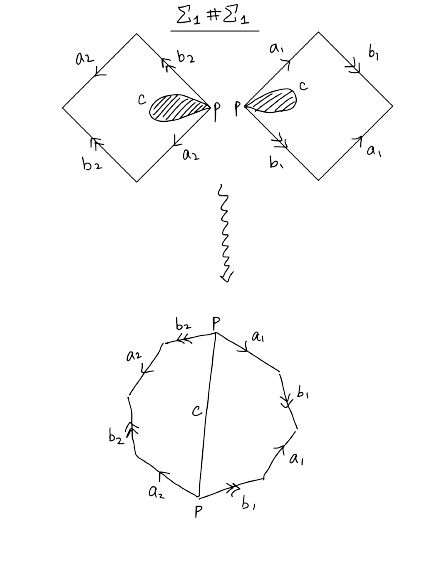
\includegraphics[scale = 0.8]{Image 1}
\end{center}

This is done by cutting a hole at the CW complex at the point $p$, and the pushing the boundary $c$ out, and then connecting them together. The cut-out hole is exactly a disc in the torus. By gluing the two toruses along the boundary $c$, we are effectively gluing the two toruses along the discs. \\~\\

The new hectagon obtained is precisely then the CW complex of $\Sigma_2$. In general, we can perform the operation of connected sum on a $(4g-4)$-gon and a square. We then obtain the CW complex of the $g$-holed torus. 

\begin{center}
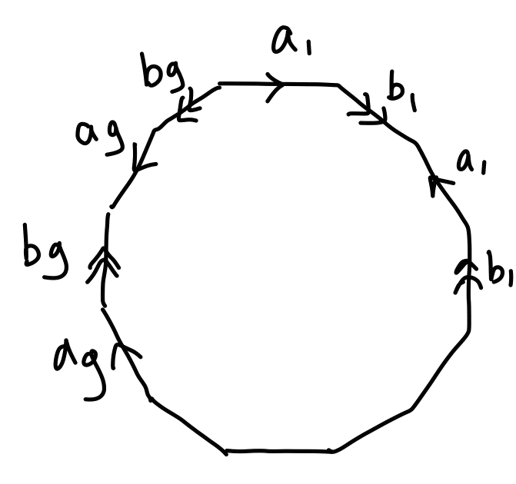
\includegraphics[scale = 0.3]{Image 2}
\end{center}

Another class of compact surfaces is the connected sum of projective spaces $\R\Prj^2$. 

\begin{defn}{Non-Orientable Surface}{} For $h\geq 1$, define $$N_h=\R\Prj^2\#\cdots\#\R\Prj^2$$ the connected sum of $h$ projective spaces. 
\end{defn}

We can do the same process of gluing the CW complexes just like that of the torus to obtain the $4h$-gon that represents $N_h$: 

\begin{center}
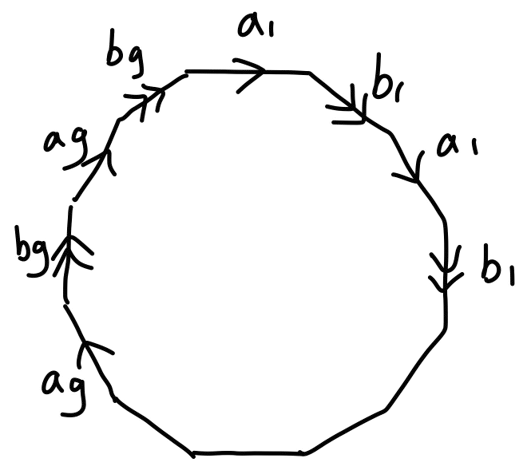
\includegraphics[scale = 0.3]{Image 3}
\end{center}

It is also meaningful to ask what would happen if we perform connected sums through the two class of compact surfaces. We obtain the following. 

\begin{prp}{}{} Let $N_3$ denote the connected sum of three projective spaces $\R\Prj^2$. Then we have that $$T\#\R\Prj^2=N_3$$ 
\end{prp}

The above two classes of compact surfaces together with the sphere exhausts all possible cases for compact surfaces. 

\begin{thm}{}{} Every compact surface is homeomorphic to exactly one of the following. 
\begin{itemize}
\item $\Sigma_g$ for $g\geq 0$
\item $N_h$ for $h\geq 1$
\end{itemize}
\end{thm}

\subsection{Homology and Cohomology of Compact Orientable Surfaces}
\begin{prp}{}{} Let $g\geq 0$. The homology of the $g$-holed torus $\Sigma_g$ is given by $$H_n(\Sigma_g)=\begin{cases}
\Z & \text{ if } n=0,2\\
\Z^{2g} & \text{ if } n=1\\
0 & \text{otherwise}
\end{cases}$$ \tcbline
\begin{proof}
Cut an open disc along the middle of the CW complex as follows

\begin{center}
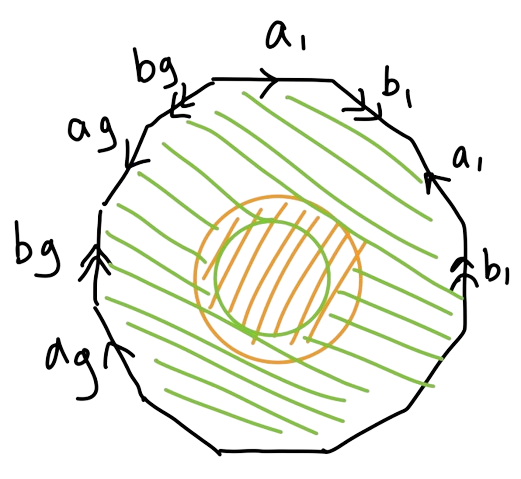
\includegraphics[scale = 0.3]{Image 4}
\end{center}

and label it $V$ (the orange part). Label the green part as $U$. It is clear that $U\cap V\simeq S^1$, $U$ is contractible and $V$ deformation retracts to the boundary, which is actually just a wedge sum of $2g$ circles. By the formula for the homology of wedge sums we have that $$H_n(V)=\begin{cases}
\Z & \text{ if } n=0\\
\Z^{2g} & \text{ if } n=1\\
0 & \text{ otherwise }
\end{cases}$$ By the reduced Mayer-Vietoris sequence, the only non-trivial homology groups in the sequence are \\~\\
\adjustbox{scale=1.0,center}{\begin{tikzcd}
	0 & {\widetilde{H}_2(\Sigma_g)} & \Z & {\Z^{2g}} & {\widetilde{H}_1(\Sigma_g)} & 0
	\arrow[from=1-1, to=1-2]
	\arrow[from=1-2, to=1-3]
	\arrow[from=1-3, to=1-4]
	\arrow[from=1-4, to=1-5]
	\arrow[from=1-5, to=1-6]
\end{tikzcd}}\\~\\
and the exact sequence \\~\\
\adjustbox{scale=1.0,center}{\begin{tikzcd}
	0 & {\widetilde{H}_0(\Sigma_g)} & 0
	\arrow[from=1-1, to=1-2]
	\arrow[from=1-2, to=1-3]
\end{tikzcd}}\\~\\
in which the latter immediately shows that $H_0(\Sigma_g)\cong\Z$. Now the map $\Z\to\Z^{2g}$ sends a generator of the first homology of $U\cap V\simeq S^1$ to the loop $$a_1+b_1-a_1-b_1+\cdots+a_g+b_g-a_g-b_g$$ Since $\Z^{2g}$ is abelian, we conclude that this map is actually the zero map. It follows that $H_2(\Sigma_g)\cong\Z$ and $H_1(\Sigma_g)\cong\Z^{2g}$. 
\end{proof}
\end{prp}

We can immediate deduce the orientability of $\Sigma_g$ using the machinery in section $1$. 

\begin{crl}{}{} The surfaces $\Sigma_g$ for $g\geq 0$ is orientable. \tcbline
\begin{proof}
By the above, we have that $H_2(\Sigma_g)\cong\Z$. The long exact sequence for relative homology groups give \\~\\
\adjustbox{scale=0.9,center}{\begin{tikzcd}
	\cdots & {H_2(\Sigma_g\setminus\{x\})} & {H_2(\Sigma_g)} & {H_2(\Sigma_g,\Sigma_g\setminus\{x\})} & {H_1(\Sigma_g\setminus\{x\})} & {H_1(\Sigma_g)} & \cdots
	\arrow[from=1-1, to=1-2]
	\arrow[from=1-2, to=1-3]
	\arrow[from=1-3, to=1-4]
	\arrow[from=1-4, to=1-5]
	\arrow[from=1-5, to=1-6]
	\arrow[from=1-6, to=1-7]
\end{tikzcd}}\\~\\
Let $U$ be as the proof above. Then the inclusion from $U$ to $\Sigma\setminus\{x\}$ is a homotopy equivalence. Moreover, $\Sigma\setminus\{x\}$ is a $2g$-fold wedge of circles labelled $a_1,b_1,\dots,a_g,b_g$ and $H_2(\Sigma_g\setminus\{x\})=0$. Also, we have that $H_1(U)\cong H_1(\Sigma_g)$ from above and hence $H_1(\Sigma_g\setminus\{x\})\cong H_1(\Sigma_g)$. The last map is invertible so that by exactness, the third map is the zero map. Then what remains is an isomorphism $$H_2(\Sigma_g)\cong H_2(\Sigma_g,\Sigma_g\setminus\{x\})$$ Now since this isomorphism factors through $H_2(\Sigma_g,\Sigma_g\setminus B)$ for any ball $B$ containing $x$, we thus have a consistent local orientation throughout all of $\Sigma_g$. 
\end{proof}
\end{crl}

\begin{prp}{}{} Let $g\geq 0$. Let $A$ be an abelian group. The singular cohomology of the $g$-holed torus $\Sigma_g$ with coefficients in $A$ is given by $$H^n(\Sigma_g;A)=\begin{cases}
A & \text{ if } n=0,2\\
A^{2g} & \text{ if } n=1\\
0 & \text{otherwise}
\end{cases}$$ \tcbline
\begin{proof}
Applying the universal coefficient theorem easily gives all the required cohomology groups. 
\end{proof}
\end{prp}

We use the cohomology of $\Sigma_g$ to illustrate generators of cohomology. Ref: Hatcher Ex3.7. 

\begin{prp}{}{} Let $g\geq 0$. The integral cohomology ring of $\Sigma_g$ is given by $$H^\ast(\Sigma_g;\Z)\cong\frac{\Z[\alpha_1,\beta_1,\dots,\alpha_g,\beta_g]}{(\alpha_i^2,\beta_i^2,\alpha_i\alpha_j,\beta_i\beta_j,\alpha_i\beta_j,\beta_i\alpha_j,\alpha_i\beta_i+\beta_i\alpha_i\;|\;1\leq i\neq j\leq g)}\cong\Lambda^2(\Z^{2g})$$ where each $\alpha_i$ and $\beta_i$ are of degree $1$ in the graded ring. \tcbline
\begin{proof}
Consider the following CW complex of $\Sigma_g$. Recall that a basis for $H_1(\Sigma_g)$ is given by $a_1,b_1,\dots,a_g,b_g$. Consider the dual basis $\alpha_1,\beta_1,\dots,\alpha_g,\beta_g$. By definition these are precisely the generators of $H^1(\Sigma_g;\Z)$. By definition the value of $\alpha_i$ is $1$ on $a_i$ and $0$ otherwise. This is similar for $\beta_i$. We want to find elements of $Z^1(\Sigma_g;\Z)$ that represent $\alpha_i$ and $\beta_i$. Consider the following diagram: Define $\phi_i\in C^1(\Sigma_g;\Z)$ to be the map that gives $1$ for any edge that intersects with $s_i$ and $0$ otherwise. Similarly, define $\psi_i:\in C^1(\Sigma_g;\Z)$ to be the map that gives $1$ for any edge that intersects with $t_i$ and $0$ otherwise. It is easy to see that $\delta(\phi_i)=0$ and $\delta(\psi_i)=0$ so that $\phi$ and $\psi$ are indeed cocycles. Moreover, they represent $\alpha_i$ and $\beta_i$ respectively. \\~\\

Now notice that I have indicated orientations for each $2$-simplices in $\Sigma_g$ depending on whether they are oriented clockwise or anti-clockwise. Define an element of $C_2(\Sigma_g)$ by the sum of the $2$-simplices with $\pm1$ as their coefficient depending on their orientation. It is easy to see that the sum is a $2$-cycle that generates $H_2(\Sigma_g)$. Let $\gamma$ be its dual generator. \\~\\

It is easy to check that $$\phi_i\smile\psi_j=-\psi_j\smile\phi_i=\begin{cases}
\gamma & \text{ if }i=j\\
0 & \text{ otherwise}
\end{cases}$$
and $\alpha_i\smile\alpha_j=\beta_i\smile\beta_j=0$ for $1\leq i,j\leq g$. We conclude that the cohomology ring of $\Sigma_g$ is given by desired form. 
\end{proof}
\end{prp}

\subsection{Homology and Cohomology of Compact Non-Orientable Surfaces}
\begin{prp}{}{} Let $h\geq 1$. The homology of $N_h$ is given by $$H_n(N_h)=\begin{cases}
\Z & \text{ if } n=0\\
\Z^{h-1}\oplus\Z/2\Z & \text{ if } n=1\\
0 & \text{otherwise}
\end{cases}$$ \tcbline
\begin{proof}
Similar to the proof in that of $\Sigma_g$, cut an open disc along the middle of the CW complex of $N_h$ as follows 

\begin{center}
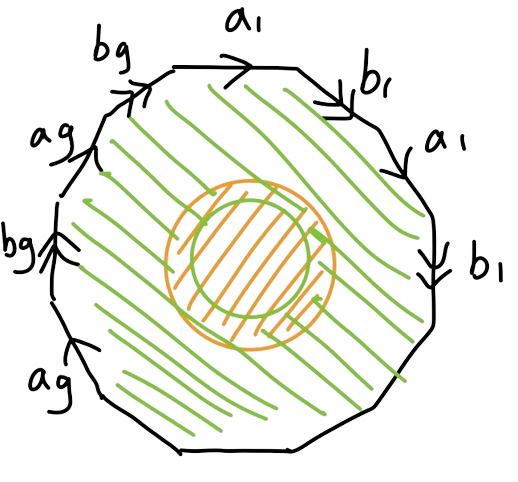
\includegraphics[scale = 0.3]{Image 5}
\end{center}

and again label the green part $U$ and the orange part $V$. Then apply Mayer-Vietoris sequence to acquire a similar exact sequence \\~\\
\adjustbox{scale=1.0,center}{\begin{tikzcd}
	0 & {\widetilde{H}_2(\Sigma_g)} & \Z & {\Z^h} & {\widetilde{H}_1(\Sigma_g)} & 0
	\arrow[from=1-1, to=1-2]
	\arrow[from=1-2, to=1-3]
	\arrow[from=1-3, to=1-4]
	\arrow[from=1-4, to=1-5]
	\arrow[from=1-5, to=1-6]
\end{tikzcd}}\\~\\
together with $\widetilde{H}_0(N_h)\cong 0$. Notice that the third non-zero term counting from the left is now $\Z^h$ instead of $\Z^{2g}$ as in the torus because the boundary circle is the wedge sum of $h$ circles labelled $a_1b_1,\dots,a_hb_h$. The map $\Z$ to $\Z^h$ is now given by sending the generator $1$ to $$2(a_1+b_1+\dots+a_h+b_h)$$ The Smith Normal form of the matrix is an $h\times 1$ matrix with $2$ at the first entry and $0$ everywhere else. In particular, it means that this map is injective so that $\widetilde{H}_2(N_h)\to\Z$ is the $0$ map so that $\widetilde{H}_2(N_h)\cong 0$. Now it remains an exact sequence \\~\\
\adjustbox{scale=1.0,center}{\begin{tikzcd}
	0 & \Z & {\Z^h} & {\widetilde{H}_1(N_h)} & 0
	\arrow[from=1-1, to=1-2]
	\arrow[from=1-2, to=1-3]
	\arrow[from=1-3, to=1-4]
	\arrow[from=1-4, to=1-5]
\end{tikzcd}}\\~\\
The image of the matrix is $2\Z$ and by exactness this is the kernel of the map $\Z^h\to\widetilde{H}_1(N_h)$. Thus we have an isomorphism $$\widetilde{H}_1(N_h)\cong\Z^{h-1}\oplus\Z/2\Z$$ and so we conclude. 
\end{proof}
\end{prp}

\begin{crl}{}{} The surfaces $N_h$ for $h\geq 1$ is non-orientable. \tcbline
\begin{proof}
Notice that removing a small closed disk from $\R\Prj^2$ yields a space homeomorphic to the open Mobius strip. It follows that for $h>0$, the space $N_h$ contains the open Mobius strip as a subspace. Since the Mobius strip is non-orientable, $N_h$ is also non-orientable. 
\end{proof}
\end{crl}

\begin{prp}{}{} Let $h\geq 1$. The singular cohomology of non-orientable surface $N_h$ with coefficients in $\Z$ is given by $$H^n(N_h;\Z)=\begin{cases}
\Z & \text{ if } n=0\\
\Z^{h-1} & \text{ if } n=1\\
\Z/2\Z & \text{ if } n=2\\
0 & \text{otherwise}
\end{cases}$$ \tcbline
\begin{proof}
We use the universal coefficient theorem in all dimensions. 
When $n=0$, we have that 
\begin{align*}
H^0(N_h;\Z)&\cong\Hom(H_0(N_h;R);\Z)\oplus\text{Ext}(H_{-1}(N_h;\Z),\Z)\\
&\cong\Hom(\Z,\Z)\oplus 0\\
&\cong\Z
\end{align*}
When $n=1$, we have that 
\begin{align*}
H^1(N_h;\Z)&\cong\Hom(H_1(N_h),\Z)\oplus\text{Ext}(H_0(N_h),\Z)\\
&\cong\Hom(\Z^{h-1}\oplus\Z/2\Z,\Z)\oplus\text{Ext}(\Z,\Z)\\
&\cong\Z^{h-1}\oplus 0\\
&\cong\Z^{h-1}
\end{align*}
When $n=2$, we have that 
\begin{align*}
H^2(N_h;\Z)&\cong\Hom(H_2(N_h),\Z)\oplus\text{Ext}(H_1(N_h),\Z)\\
&\cong\Hom(\Z,\Z)\oplus\text{Ext}(\Z^{h-1}\oplus\Z/2\Z,\Z)\\
&\cong 0\oplus\text{Ext}(\Z^{h-1},\Z)\oplus\text{Ext}(\Z/2\Z,\Z)\\
&\cong 0\oplus 0\oplus \Z/2\Z\\
&\cong\Z/2\Z
\end{align*}
When $n\geq 3$, we have that 
\begin{align*}
H^n(N_h;\Z)&\cong\Hom(H_n(N_h),\Z)\oplus\text{Ext}(H_{n-1}(N_h),\Z)\\
&\cong\Hom(0,\Z)\oplus\text{Ext}(0,\Z)\\
&\cong 0
\end{align*}
and so we conclude. 
\end{proof}
\end{prp}

\begin{prp}{}{} Let $h\geq 1$. Then there is a graded ring isomorphism $$H^\ast(N_h;\Z)\cong\frac{\Z[\alpha_1,\dots,\alpha_h]}{(\alpha_i^3,\alpha_i\alpha_j,\alpha_i^2-\alpha_j^2\;|\;1\leq i\neq j\leq n)}$$ where each $\alpha_i$ has degree $1$. 
\end{prp}

\subsection{The Euler Characteristic}
\begin{crl}{}{} For $g\geq 0$ and $h>1$, the Euler characteristic of any compact surface is given by $$\chi(\Sigma_g)=2-2g\;\;\;\;\text{ and }\;\;\;\;\chi(N_h)=2-h$$ \tcbline
\begin{proof}
It follows directly by repeated applications of the above corollary. 
\end{proof}
\end{crl}

Recall that if $p:\widetilde{X}\to X$ is a $d$-sheeted covering and $X$ is a finite CW complex, then we have the formula $$\chi(\widetilde{X})=d\cdot\chi(X)$$

\pagebreak
\section{Higher Dimensional Manifolds}
\subsection{Manifolds of Dimension 3}
\begin{thm}{}{}
\end{thm}
















\end{document}
